\section{Simulation Results and Discussion}
\subsection{Constant food and egg laying}
\label{chap:constantFoodConstantLaying}
The first iterative simulation run is based only on the equations of \textit{David S. Khoury et al.}\cite{khoury13}. As expected the hive stabilizes at a equilibrium point while the stored food increases infinite. (See graph \ref{chap:sim_R0_1})
\subsection{Constant food, dynamic egg laying}
\label{chap:constantFoodDynamicLaying}
The second iterative simulation run was to see if the new laying function (Figure \ref{fig:dynLayingRate})  was working as intended. As a result the bee population does not stabilize at one point, it now describes a more natural periodic form with a population maximum around August and a minimum around February. The stored food still increases infinite but now the correlation between the number of forager bees and the daily increase in stored food is very to see (linear correlation coefficient =  0.9775).

\subsection{Environmental model}
	\subsection{Empirical data based run}
	In this run we wanted to see if our model can produce the same results as \textit{T.D. Seeley's} experiments from \textit{Wisdeom of the hive} pp.44 fig. 2.14. Our date correlates quite well with the empirical data before swarming occurs, year 1982 compared to graph \ref{chap:sim_R1_1}. As swarming was never a part of our model were satisfied with the accuracy of our model.	
	Compared to our earlier simulations, the food collection rate is now dominated by the availability of flowers. The forager count is still a important factor as later simulations will show.
	\subsubsection{Typical simulated day}
			\begin{figure}
				\centering
				\scalebox{.75}{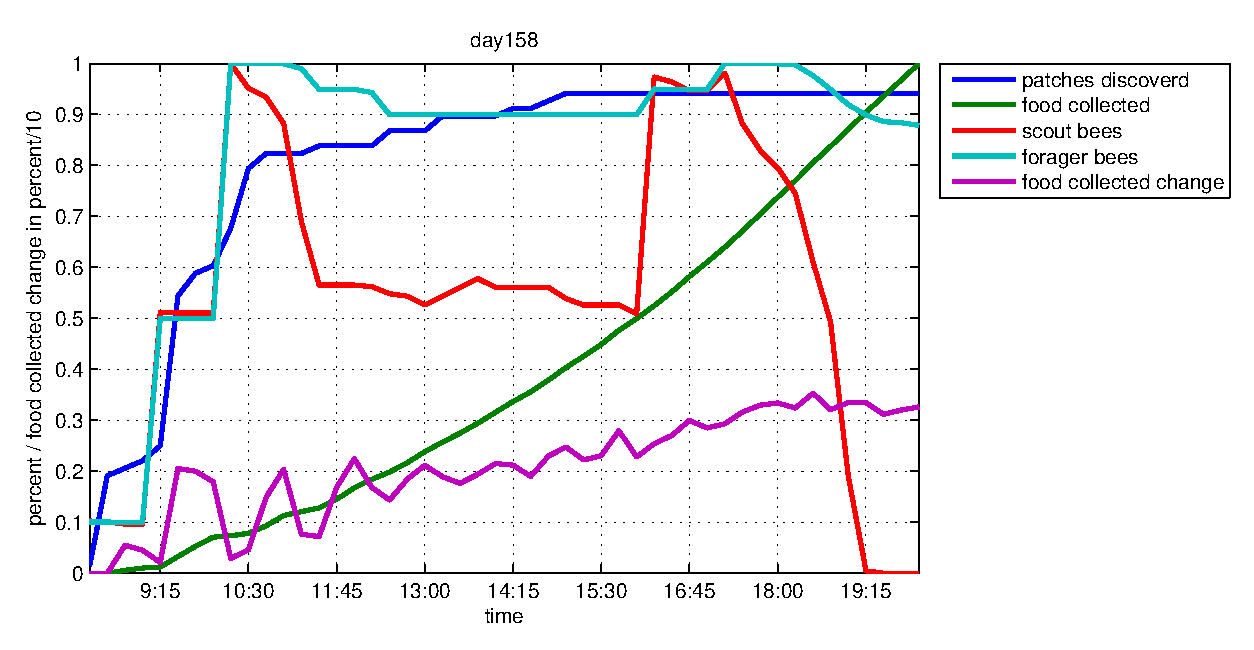
\includegraphics{../../code/results/Properties_Base_R1_1_day158.eps}}
				\caption{\textit{A summer day from the standard run R1\char`_1}}
				\label{fig:day158}
			\end{figure}
	 
	%TODO /PLANNED a summer day video / pictures	
	\subsubsection{Missing flower seasons}
	% summer and fall essential
	\subsubsection{Variations on autumn flowers}
	% we'll see what i find outd
